\subsection*{Appendix A.1}

We need to build up the idea of consumer preferences and taste.
If we compare the quantity of good 1 and good 2, any point or bundle
will provide a certain level of utility. From this bundle, we can compare
utility levels for other bundles. The curve of all points that give the same
level of utility is the idea of an \emph{indifference curve}. There is 
an infinite number of indifference curves for two goods. Extremes are unfavoured.
\begin{enumerate}
    \item The further/highest
    the indifference curve, the higher the utility.
    \item Indifference curves must be downward 
    sloping.
    \item Indifference curves cannot intersect.
    \item Indifference curves must be convex (bow out).
    \item The slope of the indifference curve is -$\frac{MU_1}{MU_2}$ or -MRS.
\end{enumerate}
\begin{figure}[H]
    \centering
    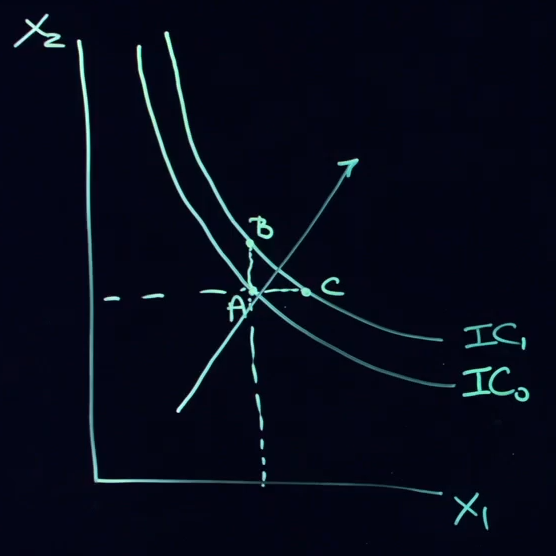
\includegraphics[width=0.5\textwidth]{Chapter6/IndifferenceCurve.png}
    \caption{Indifference Curve}
    \label{fig:Indifference_Curve}
\end{figure}